\documentclass[compress]{beamer}
\useoutertheme[footline=authorinstitutetitle]{miniframes}
\usecolortheme{whale}
\usecolortheme{orchid}
\useinnertheme{rounded}

\setbeamerfont{block title}{size={}}

%\usepackage{beamerthemeproyxetex}
%\usepackage{synttree}

\title{COLIBRI: Constructions as Linguistic Bridges}
\author{Maarten van Gompel}
\date{December 2011}
\usepackage{graphicx}
\usepackage{placeins}



\def\raccoon{
\makebox[\linewidth][c]{\includegraphics[width=70pt]{/home/proycon/Pictures/All/raccoon.pdf}\FloatBarrier}
}
\def\smallraccoon{
\makebox[\linewidth][c]{\includegraphics[width=30pt]{/home/proycon/Pictures/All/raccoon.pdf}\FloatBarrier}
}

\begin{document}

\begin{frame}
	\titlepage\smallraccoon
\end{frame}

\section{Introduction}

\begin{frame}

	\begin{block}{Background information}
		\begin{itemize}
			\item \emph{2008-2009}: Master student Human Aspects of Information Technology at Tilburg University
			\item \emph{2009-2011}: Scientific programmer at Tilburg University
			\item \emph{2011--}: PhD researcher at RU since September 2011
		\end{itemize}
	\end{block}

	\begin{block}{My field}
		\begin{itemize}
			\item Language Technology
			\begin{itemize}
				\item Implicit Linguistics
				\item Machine Learning
				\item Machine Translation
			\end{itemize}
		\end{itemize}
	\end{block}

\end{frame}



\begin{frame}{Translation is hard}

	\begin{example}{Automated translation is difficult!}

		\textbf{Nederlands:} De PVV wil fors korten op ontwikkelingssamenwerking. De peiling van De Hond geeft aan dat slechts 4 procent van zijn achterban dat absoluut niet wil. Bijna een op de vijf CDA-stemmers is daar echt niet voor te vinden, terwijl voor het CDA in de Tweede Kamer verlagen van ontwikkelingshulp moeilijk ligt.  \texttt{(bron: nu.nl)} \\

		\smallskip

		\textbf{Google Translate:} 
		The PVV will considerably shorten the development. The poll of Dog indicates that only 4 percent of his supporters that absolutely does not want. Nearly one in five voters CDA is really not to be found, while the Christian Democrats in the House reduction of development is difficult. \\

	\end{example}

\end{frame}



\begin{frame}{Translation is hard}

	\begin{block}{Naive word-by-word? No}
		\begin{tabular}{cccccc}
			I & see &  & a & poor & man \\
			 & Veo & a & un & hombre & pobre \\
		\end{tabular}	
	\end{block}

	\begin{block}{Idioms}
		\begin{itemize}
			\item It's a piece of cake!
			\item Het is een stukje taart!
			\item Het is een peulenschil!
			\item It's a pea shell!
		\end{itemize}
	\end{block}
	
\end{frame}

\begin{frame}{Translation is hard}
	\begin{block}{Ambiguity}

		\begin{itemize}
			\item Mijn geld staat op de \textbf{bank} 
			\item My money is in the \textbf{bank}
		\end{itemize}

		\begin{itemize}
			\item Mijn geld ligt in een doosje onder de \textbf{bank}
			\item My money is in a box under the \textbf{sofa}
		\end{itemize}

		\begin{itemize}
			\item My boat is on the \textbf{bank} of the river
			\item Mijn boot ligt aan de \textbf{oever} van de rivier
		\end{itemize}	
	\end{block}
\end{frame}

\section{Machine Translation}

\begin{frame}
	\begin{block}{Approaches}
		\begin{enumerate}
			\item \textbf{Rule-based:} explicit linguistic knowledge
			\item \textbf{Data-driven:} implicit linguistics	
			\begin{itemize}
				\item Statistical models
				\item Memory-based machine learning
			\end{itemize}						
		\end{enumerate}
	\end{block}

	\begin{block}{Two important aspects of translation}
		\begin{enumerate}
			\item Faithful conservation of meaning
			\item Fluent natural style
		\end{enumerate}
	\end{block}

	\begin{block}{These can be modelled}
		\begin{enumerate}
			\item Faithful conservation of meaning: $argmax_T P(T|S)$
			\item Fluent natural style: $argmax_T P(T)$
			\item $besttranslation_T = argmax_T P(T) \cdot P(T|S)$
		\end{enumerate}
	\end{block}
\end{frame}


\begin{frame}
	\begin{block}{What are the units of translation? $\rightarrow$ constructions }
		\begin{itemize}
			\item Whole sentences at once? No \\
			\item Single words, word by word? No \\
			\item Words in context? Better \\
			\item Variable-length phrases in context? Even better \\
			\item Loosening constraints: ``constructions'' in context? Best? \\
		\end{itemize}
	\end{block}

	\begin{center}
		 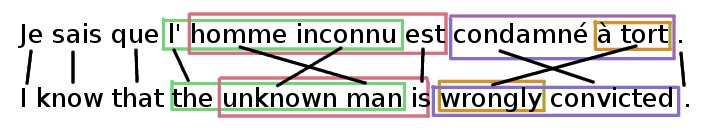
\includegraphics[width=90.0mm]{pbmbmt_alignment1c.jpg} \\
		 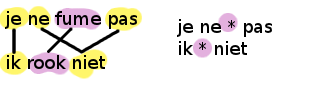
\includegraphics[width=50.0mm]{skipgram.png}
	\end{center}
\end{frame}


\section{Constructions}

\begin{frame}
	\begin{block}{What is a construction?}
		\textbf{First stage of research:}  \\
		\emph{The identification and extraction of ``good'' constructions from corpus data} \\
		We are looking for the intuitive ``atom'' in memory-based machine translation. A level above n-gram models and below syntactic level. \\
		\smallskip
		\textbf{What is a construction?}  \\
		\begin{itemize}
			\item A \emph{pattern} of words, possibly with ``skips'', which in some way forms an entity
			\item Constructions emerge from the data (parallel corpora) rather than linguistic theory:
			\begin{enumerate}
				\item by frequency
				\item by subsumption
				\item by multilingual alignment
			\end{enumerate}
		\end{itemize}
	\end{block}
\end{frame}

\begin{frame}
	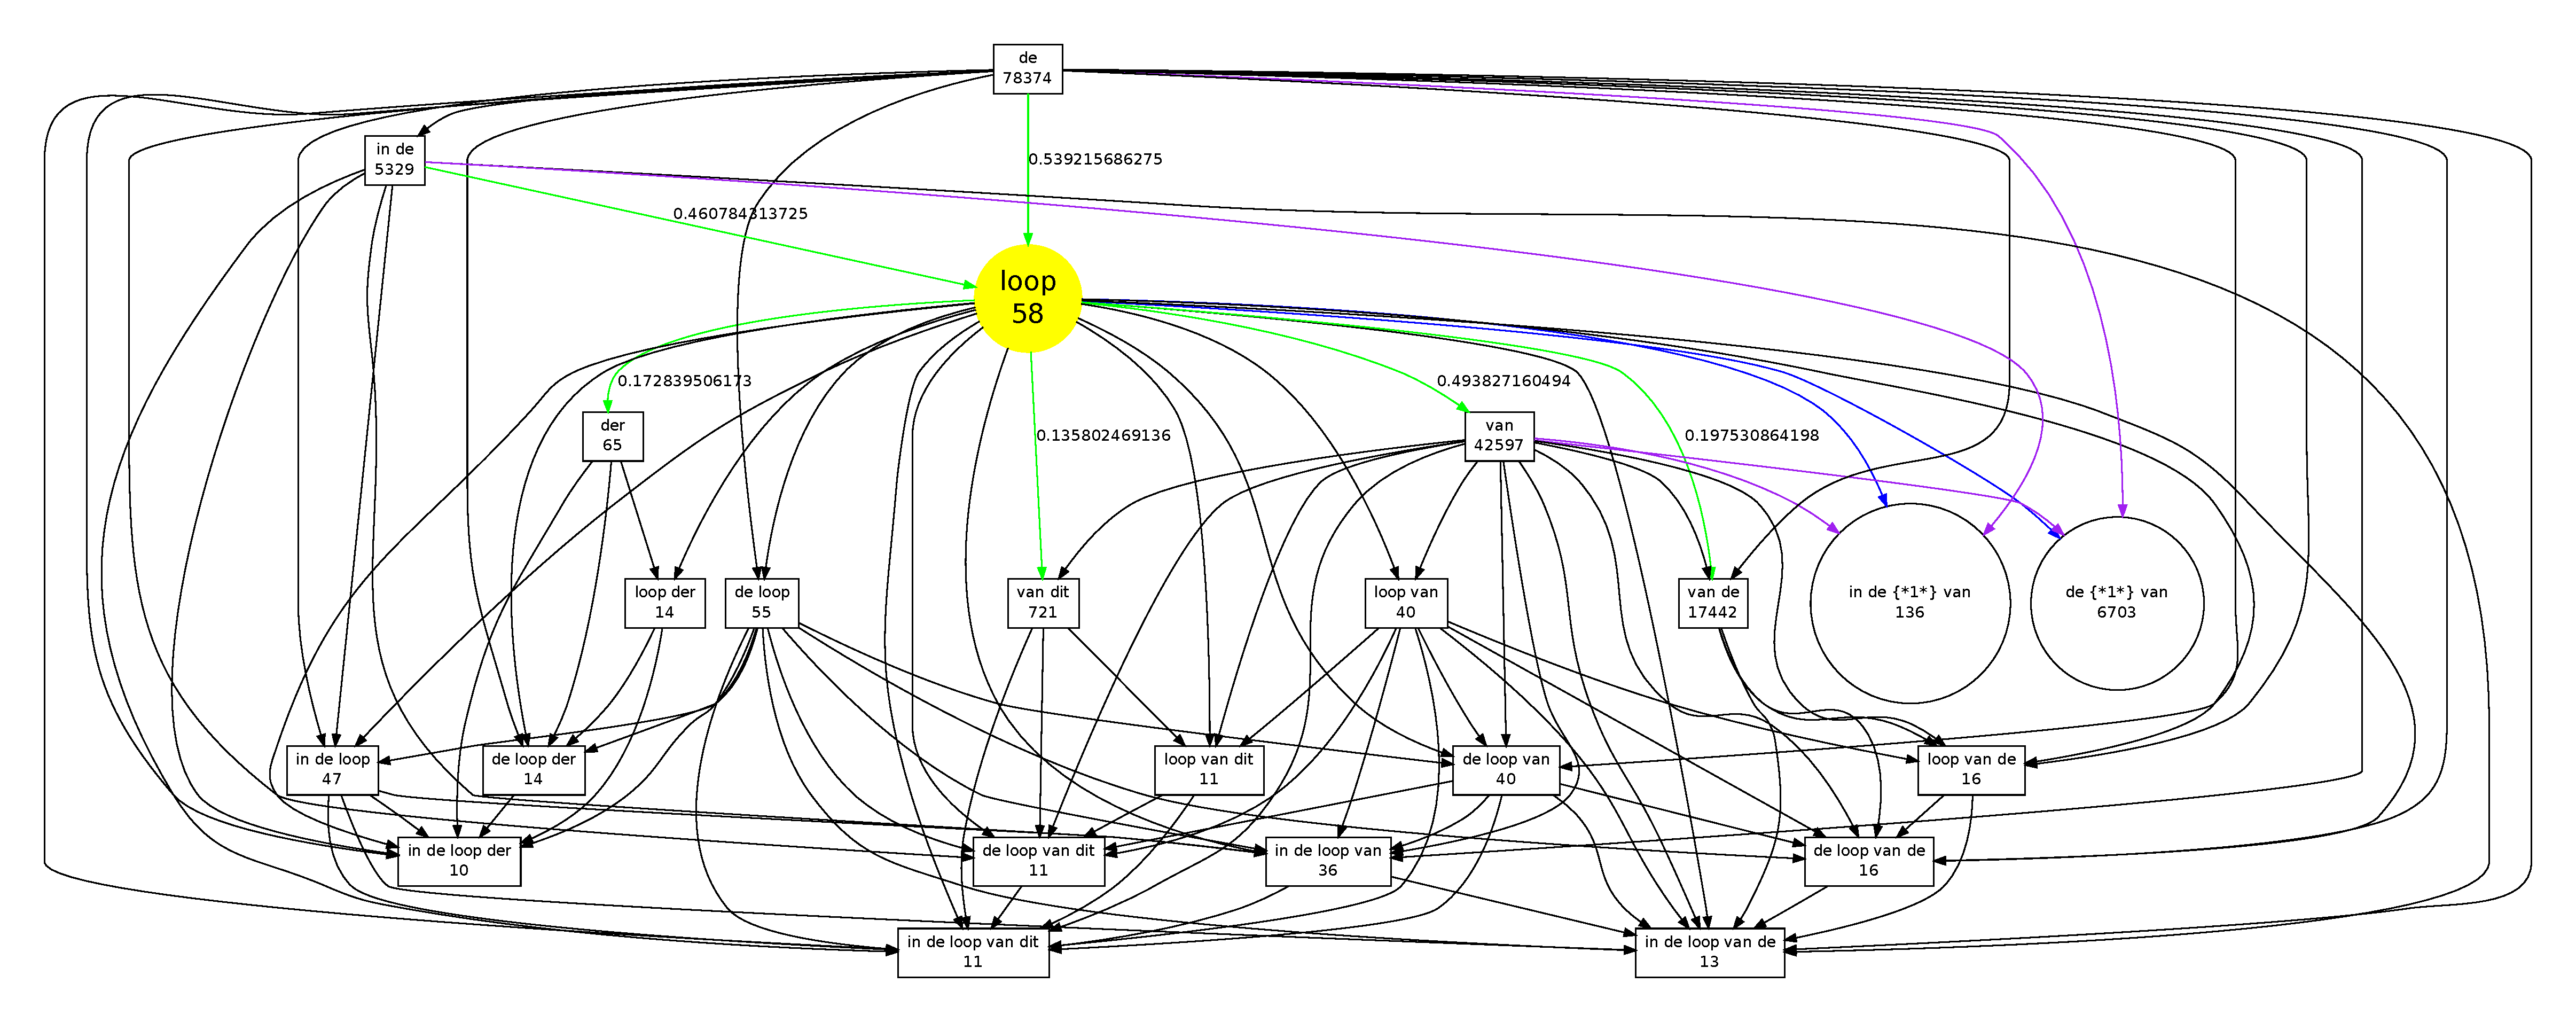
\includegraphics[width=120.0mm]{patterngraph4.pdf}
\end{frame}


\section{Alignment}

\begin{frame}[fragile]
	\begin{block}{Aligning constructions}
		\textbf{Second  stage of research:}  \\
			\emph{Establishing aligned constructions, a mapping between constructions in two (or more) languages} \\		

		\textbf{How?} \emph{Measures of co-occurrence} \\
	\end{block}

	\begin{example}	
		\begin{tabular}{|l|l|}
			\hline
			'Uraa al-kalba & I see the dog			\\
			'Uraa al-qitta & I see the cat			\\
			akala al-kalbu & The dog ate				 \\
			Yaqtulu al-kalbu al-qitta &  The dog kills the cat \\
			\hline
		\end{tabular} \\
		Try now: \emph{'uraa? al-kalbu? al-qitta? akala? yaqtulu? al? }
	\end{example}
\end{frame}

\section{Machine learning}

\begin{frame}
	\begin{block}{Machine Learning - Construction experts}
		\textbf{Third stage:} \emph{Local translation step} \\

		Once we have alignments, can we build automated classifiers that 'predict' the translation of constructions? \\
		\textbf{Hypothesis:} Construction-experts, one classifier for each construction, increase translation accuracy. \\ %proven in WSD
		\smallskip
		Predicted translation is made on the basis of to-be-determined features, such as context.
	\end{block}

	\begin{center}
		 
\includegraphics[width=90.0mm]{presinstance2.png} \\		
	\end{center}
\end{frame}

\section{Decoding}

\begin{frame}
	\begin{block}{Decoding}

		\textbf{Fourth stage:} \emph{Global translation step -- Decoding} \\

		\begin{itemize}
			\item \textbf{search problem:} Recombine translated constructions into coherent translations in the target language.		
			\item Translation hypothesis are scored using some kind of evaluation function
		\end{itemize}

    	 %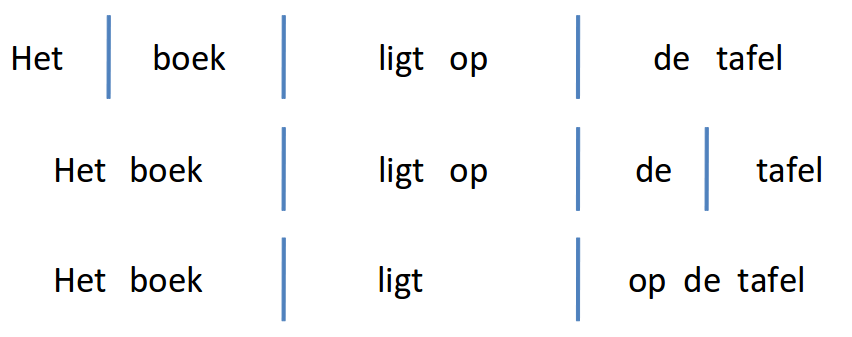
\includegraphics[width=90.0mm]{fragmentations.png}

	\end{block}

	\begin{center}
		 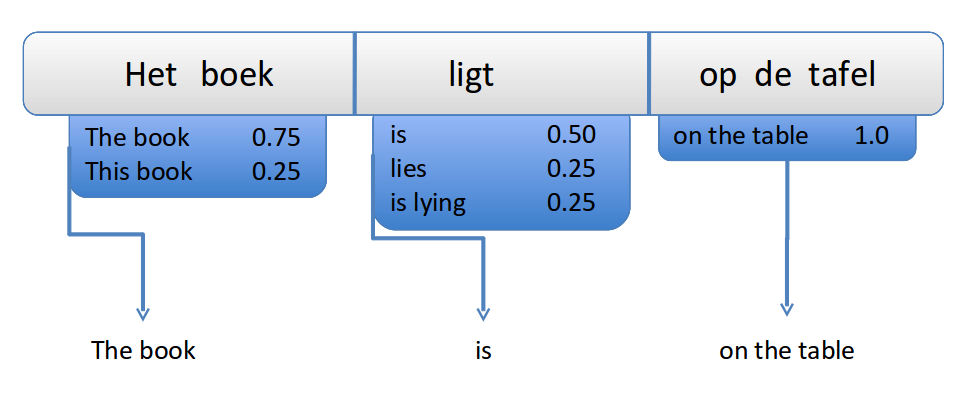
\includegraphics[width=60.0mm]{decoder1.png} 
		 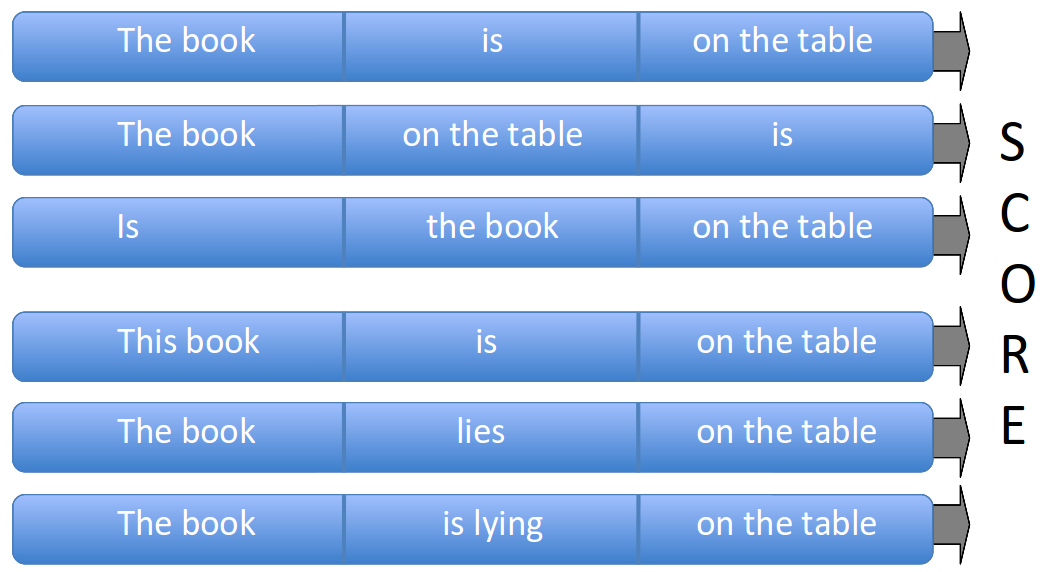
\includegraphics[width=50.0mm]{decoder_score.png} 
	\end{center}

\end{frame}


\section{Evaluation}

\begin{frame}
	\begin{block}{Evaluation}

		\begin{itemize}
			\item Full implementation needed before we can evaluate properly
			\item Evaluation of Machine Translation is not trivial.
			\begin{itemize}
				\item Comparison to human reference translations
			\end{itemize}
		\end{itemize}

	\end{block}
\end{frame}

\section{The End}

\begin{frame}

\raccoon

\begin{center}
\Large{Questions?}
\end{center}

\end{frame}


\end{document}  

